\documentclass[12pt]{article}
\usepackage{fullpage,enumitem,amsmath,amssymb,graphicx}
\usepackage{listings} % This is a package for including code in your solution.
\usepackage{graphicx} % This is a package for including graphics in your solution.

\title{CS168 Spring Assignment 1}
\author{
	Yueyao Zhu	(yyzhu@stanford.edu) \\
	Yang Du (yd322@stanford.edu)
}

\begin{document}
\maketitle

\section*{Honor Code}

By turning in this assignment, I agree by the Stanford honor code and declare
that all of this is my own work.

\section*{Part 1}

\begin{enumerate}[label=(\alph*)]
 	\item (See code \textbf{simu.py})
 	\item (See \textbf{Figure~\ref{fig:plot}})
	\item 

The placement of the balls into the bins is analogious compare to the hashing with chaining. Placing one ball into a bin, is like put a new object into a bucket where the bucket number is the hash value. The number of balls in the bins, is compared to the number of chaining objects in the bucket. 

The first strategy suggests us to implement the hashing using one hash function, and put the object into the box indicated by its hash value

The second strategy suggests us to use two hash functions. And look how many objects are in each buckets, and put the new object in the bucket with less objects in it.

The third strategy suggests us to use three hash functions using the above strategy.
The fourth strategy suggests us to make two separate region for the hash buckets. And we use two different hash functions. And we place the new object in the bucket where the bucket contains less objects.

The first strategy is the most common one we used. It is very possible that there will be a collision so that a bucket will contain a large amount of objects so that the time to access an objects requires a linear search on the whole chaining in the bucket.

The second strategy require one more hash function, so that for each of the new objects, it will cost the program to calculate one more times. But it will cause less collision.
The third strategy requires three hash functions so that three calculations are needed, but less collisions.
The fourth strategy either requires double space, or make each hash bucket received double elements. If we use double space, then the collision will decrease, but if we keep the space be the same, and use two hash function separately, then each bucket will have a higher chance to be hashed in.
\end{enumerate}

\begin{figure}[h]
	\centering
	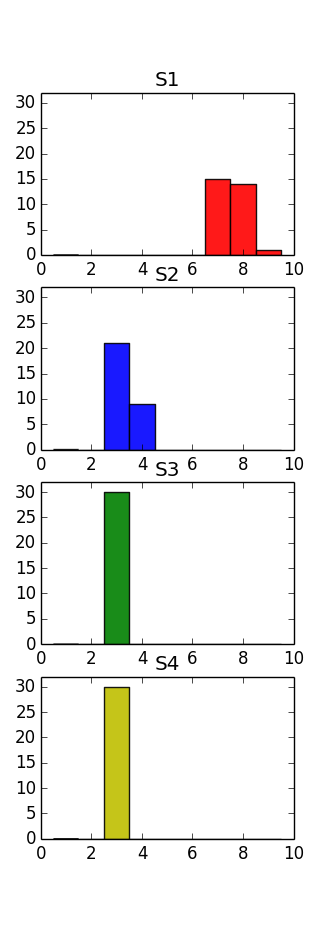
\includegraphics[width=0.4\textwidth]{figure_1.png}
	\caption{Histogram for $X$}
	\label{fig:plot}
\end{figure}

\end{document}